\documentclass[a4paper,11pt]{article}
\usepackage{ifpdf} 
\ifpdf
\pdfoutput=1 
\fi

\usepackage{jcappub}
\usepackage{graphicx}
\graphicspath{{Paper/}{./}}
\usepackage{dcolumn}
\usepackage{amssymb,amsmath,bm,bbold}
\usepackage{color}
\usepackage[dvipsnames]{xcolor}
\usepackage{xfrac}
\usepackage{aas_macros}
\usepackage{mathrsfs}
\usepackage{subcaption}
\usepackage{rotating}
\usepackage{chngcntr}
\newcommand{\nv}{\vec{\theta}}
\newcommand{\todo}[1]{{\bf TODO: #1}}

\newcommand{\as}[1]{{\textcolor{blue}{[AS: #1]}}}
\newcommand{\an}[1]{{\textcolor{magenta}{[AN: #1]}}}
\newcommand{\da}[1]{{\textcolor{red}{[DA: #1]}}}

\newcommand{\vd}{\mathbf{d}}
\newcommand{\vt}{\mathbf{t}}
\newcommand{\vN}{\mathbf{N}}

\newcommand\Tstrut{\rule{0pt}{3ex}}   

%\linenumbers

\definecolor{internationalkleinblue}{rgb}{0.0, 0.18, 0.65}
\hypersetup{urlcolor=internationalkleinblue, linkcolor=internationalkleinblue, citecolor=internationalkleinblue}

\usepackage[T1]{fontenc} % if needed
\usepackage{natbib}
\bibliographystyle{JHEP}
\title{Marginalization of photometric redshift uncertainties}

\author[a,1]{Boryana Hadzhiyska,}
\author[b]{David Alonso,}
\author[c]{Andrina Nicola,}
\author[d]{An\v{z}e Slosar,}

\affiliation[a]{Harvard-Smithsonian Center for Astrophysics, 60 Garden St., Cambridge, MA 02138, USA}
\affiliation[b]{Department of Physics, University of Oxford, Denys Wilkinson Building, Keble Road, Oxford OX1 3RH, United Kingdom}
\affiliation[c]{Department of Astrophysical Sciences, Princeton University, Peyton Hall, Princeton NJ 08544-0010, USA}
\affiliation[d]{Brookhaven National Laboratory, Physics Department, Upton, NY 11973, USA}
\emailAdd{boryana.hadzhiyska@cfa.harvard.edu}

\abstract{We present a new method for marginalization over uncertainties in redshift distributions of tomographic bins applicable to current and coming photometric galaxy surveys. We allow for arbitrary deviations from the best guess $N(z)$ governed by a general covariance matrix describing incompleteness in our knowledge of redshift distributions. In principle, this is marginalization over potentially hundreds of new parameters describing potential deviations as a function of redshift and tomographic bin. However, by Taylor expanding theory predictions around a fiducial model, we can perform the marginalization analytically, resulting in a modified data covariance matrix. We demonstrate  this method by applying to the galaxy clustering measurements from the Year One of Hyper SupremeCam data demonstrate how we can marginalize over sample-variance of the PZ calibration sample and a large general systematic uncertainty in photometric determination methods. We find that this method gives results that are comparable to the ad-hoc shift and width parameterizations and show that the only deviations that matter are smooth deviations. 
}


\begin{document}
\maketitle
\flushbottom

  \section{Introduction}\label{sec:intro}\label{sec:intro}
    Photometric galaxy surveys  have the potential of  being transformative in our understanding of the Universe by measuring millions and soon billions of galaxies on the sky. These catalogs can be used to constrain cosmological parameters through measurements of clustering and weak lensing as demonstrated by numerous surveys that have completed observations including  Sloan Digital Sky Survey \cite{astro-ph/0006396}, PanSTARRS \cite{2010SPIE.7733E..0EK}, Kilo-degree Survey \cite{1206.1254}, Dark Energy Survey \cite{1601.00329}, Hyper Suprime-Cam survey \cite{2012SPIE.8446E..0ZM}, and will play a crucial role in the upcoming Vera Rubin Observatory LSST Survey \cite{0912.0201}.

    it has been long recognized that the accuracy of photometric surveys relies on the accuracy of photometric redshift distributions and that these are likely to continue to be a dominant source of systematic uncertainty. The crucial quantity is the redshift distribution $N(z)$, which is simply the mean number density of galaxies as a function of redshift for each tomographic sample. It is known that the shape of $N(z)$ delivered by the current photometric redshift codes and subsequent calibrations is insufficient for retiring this source of systematic error completely \cite{1809.01669}. Improving photometric redshift techniques and calibrations is an area of active research \cite{2004.09542}\as{add citations}, but for the foreseable future we will need to rely on marginalization to control residual systematic errors.

    The traditional approach is to add nuissiance parameters that shift the best guess $N(z)$ or additionally change its width or a relative contribution from a secondary peak in $N(z)$. This usually works well, but in additional to adding potentially large number of nuissance parameters suffers from model completeness problem: how do we know that any given parameterization encompasses all possible ways in which our best-guess $N(z)$ can be wrong?

    In this paper we propose a new technique that performs a marginalization around all possible functional deviations from the best fit $N(z)$. The space of possible deviations in $N(z)$ is described as a Gaussian function and under some controlled approximations, the integrals can be performed analytically. This results in a simple change to the data covariance matrix with a simple explanation: directions in the space of predictions that are degenerate with changes in $N(z)$ are given large variance, which means that information in these direction is not used for inferring the parameters of interest. This then marginalizes over $N(z)$ uncertainty in a robust manner that does not add new niussance parameters.

    We applyt this method to the HSC data as an example and  discuss some of the advantages, limitations and possible extensions of this model. 

  \section{Theory}\label{sec:theory}
    \subsection{Redshift distribution uncertainties}\label{ssec:theory.nz}
      Most cosmological analyses involve performing Bayesian parameter inference on a posterior distribution $p(\vec{\theta} |\vd) \propto p(\vd|\vec{\theta}) p(\vec{\theta})$, where $\vd$ is a vector of data points and $\vec{\theta}$ is a set of parameters descring the underlying model.
      
      In the case of tomographic analyses of galaxy clustering and large-scale structure, $\vd$ traditionally contains correlation function or power spectrum measurements between different tracers (e.g. galaxy ellipticities or overdensity) and different redshift bins\footnote{We use the term ``redshift bin'' here to denote any given galaxy sample, whether or not it has actually been selected by binning those galaxies into intervals of some redshift estimate.}, and $\vec{\theta}$ includes both cosmological and nuisance parameters needed to produce a forward model of $\vd$ that we will call $\vt(\vec{\theta})$. Due to the central limit theorem it is often accurate enough to assume that the likelihood is Gaussian, taking the form
      \begin{equation}
        \mathcal{L} \equiv p({\bf d}|\vec{\theta}) = \frac{\exp\left [-\frac{1}{2}(\vd-\vt(\vec{\theta}))^T{\sf C}^{-1}(\vd-\vt(\vec{\theta})) \right]}{\sqrt{\det{2\pi{\sf C}}}}, \label{eq:like}
     \end{equation}
      where ${\sf C}$ is the covariance matrix of $\vd$. The information contained in the parameter dependence of ${\sf C}$ can be neglected \citep{1811.11584}, and therefore the normalization factor $\sqrt{2\pi\det{\sf C}}$ can be ignored.

      We can make significant progress without specifying explicitly how the theory is calculated given the parameters. It suffices to say that, given a set of cosmological parameters, which specify the evolution of the universe and the matter inhomogeneities as a function of scale and redshift, a set of astrophysical parameters (e.g. a particular bias or intrinsic alignment model), and the redshift distributions $N(z)$ of the different redshift bins, we can integrate these into theory predictions $\vt=\vt(\vec{\theta})$. Our main concern in this paper is the way in which the significant uncertainties in $N(z)$, which can potentially dominate the total systematic error budget, should be parametrized and marginalized over.

      The traditional approach (e.g. \todo{Add cites}) has been to parametrize departures from a given ``educated guess'' of the redshift distribution that are likely to describe the main modes in which the underlying uncertainty propagates into the theory vector. This has usually been done by introducing ``shift'' ($\Delta z$) and/or ``width'' ($z_w$) nuisance parameters, in terms of which the fiducial redshift distribution for the $i$-th redshift bin $\bar{N}_i(z)$ is modified as
      \begin{equation}
        N_{i}(z) \propto \bar{N}_{i}\left(z_{c,i} + (1 + z_{w, i})(z-z_{c, i}) + \Delta z_{i}\right), \label{eq:photo-z-model}
      \end{equation}
      where $z_{c,i}$ is the mean of the fiducial distribution and acts as a sensible pivot to define width changes. $\Delta z_i$ and $z_{w,i}$ for each bin are then inferred and marginalized over together with all other parameters, with priors on them based on calibration uncertainties.

      This approach explicitly marginalizes over two effects that are potentially the two most important systematics stemming from redshift distribution uncertainty: the width of the lens redshift distribution affects the amplitude and shape of the clustering power spectrum, and a shift in the distribution of sources influences the support of the lensing kernel and the amplitude of the shear two-point function. However, this methods suffers from two shortcomings. First, it is fundamentally ad-hoc: this particular parametric form is not directly mapped onto the main modes of uncertainty in photometric redshift estimators \todo{we may want an expert to vet this statement}, and there is rigorous proof that the parametrization is complete in the sense that it captures all relevant effects. The second problem is that it is computationally expensive. By adding one or two additional nuisance parameters per redshift bin, the dimensionality of the model parameter space increases significantly. For instance, in the analysis of \cite{1912.08209}, redshift uncertainty parameters accounted 50-60\% of all model parameters. The methodology described in the next section aims to address both of these shortcomings.

    \subsection{A new approach}\label{ssec:theory.nz_new}
      Let us consider a discretized description of the $N_i(z)$ as a sum over basis functions $\phi_\alpha(z)$:
      \begin{equation}
        N_i(z)=\sum_i N^\alpha_i\phi_\alpha(z).
      \end{equation}
      For simplicity here we will just treat $N_i(z)$ as a histogram, and therefore in our case the $\phi_\alpha$ are just top-hat functions centered on an equi-spaced grid of redshifts $z_\alpha$. The formalism described below is valid for any choice of basis functions, however. In this formalism, full set of redshift distributions is described by the vector $\vN\equiv\{N^\alpha_i\,\,\,\forall i,\alpha\}$. In what follows, we will assume that $\vN$ has units of ``counts''. The actual normalization of the $N(z)$ is irrelevant, since it only enters the theory prediction for the power spectrum as a normalized redshift probability distribution (see Eq. \todo{ref}).

      Let us further distinguish between the true underlying redshift distribution, represented by $\vN$, and a possible measurement of it $\hat{\bf N}$, with measurement uncertainties encapsulated by a covariance matrix $\hat{\sf C}_N$. Furthermore, we may have some external prior information on $\vN$, which for simplicity we will assume to be Gaussian with mean $\vN_P$ and covariance $\hat{\sf C}_P$.
      
      Our data is therefore made up of the combination ${\bf d}=(\hat{\bf c},\hat{\bf N})$, where $\hat{\bf c}$ is a set of two-point function measurements. The model parameters are $\vec{\theta}=({\bf q},\vN)$, where $\vN$ are the redsihft distribution coefficients, and ${\bf q}$ contains all other cosmological, astrophysical and nuisance parameters. The posterior distribution is therefore given by:
      \begin{align}
        p(\vec{\theta}|{\bf d})
        &=p({\bf q},\vN|\hat{\bf c},\hat{\bf N})\\\label{eq:posterior_full}
        &=p(\hat{\bf c}|{\bf q},\vN)p(\hat{\bf N}|\vN)p(\vN)p({\bf q})\\
        &=p(q)\frac{\exp\left[-\frac{1}{2}(\chi^2_c+\chi^2_N+\chi^2_P)\right]}{\sqrt{{\rm det}(2\pi{\sf C}_c){\rm det}(2\pi{\sf C}_N){\rm det}(2\pi{\sf C}_P)}},
      \end{align}
      where
      \begin{align}
        \chi^2_c&=\left(\hat{\bf c}-{\bf t}\right)^T{\sf C}_c^{-1}\left(\hat{\bf c}-{\bf t}\right)\\
        \chi^2_N&=\left(\hat{\bf N}-\vN\right)^T{\sf C}_N^{-1}\left(\hat{\bf N}-\vN\right)\\
        \chi^2_P&=\left(\vN-\vN_P\right)^T{\sf C}_P^{-1}\left(\vN-\vN_P\right),
      \end{align}
      and ${\bf t}(q,\vN)$ is the theoretical prediction for $\hat{\bf c}$.
      
      In Eq. \ref{eq:posterior_full} we have assumed that $\hat{\bf c}$ and $\hat{\vN}$ are independent at the likelihood level, and that the likelihood of $\hat{\vN}$ is independent of ${\bf q}$. The validity of these assumptions should be studied in detail, especially in cases where $\vN$ is calibrated using a spectroscopic sample with significant spatial overlap with the data under study (through a clustering redshifts approach \todo{cite} or otherwise). The method outlined here is still applicable if these assumptions are dropped, albeit with a different expression for the modified covariance in Eq. \ref{eq:main2}. We have also assumed that the redshift distribution amplitudes $\hat{\vN}$ are Gaussianly distributed. \todo{add some blab here and potentially cite Carles Sanchez's latest paper.}

      To derive the main result of this paper, let us start by considering the combination $\chi^2_N+\chi^2_P$. After completing squares for $\vN$, this can be written as:
      \begin{equation}
        \chi^2_N+\chi^2_P\equiv\chi^2_{\bar{N}}=\left(\vN-\tilde{\vN}\right)^T{\sf P}^{-1}\left(\vN-\tilde{\vN}\right)+K_N,
      \end{equation}
      where we have defined the \emph{smoothed mean} $\bar{\vN}$ and combined prior covariance ${\sf P}$ as:
      \begin{align}\label{eq:priorcov}
        \bar{\vN}\equiv{\sf P}({\sf C}_N^{-1}\hat{\bf N}+{\sf C}_P^{-1}\vN_P),\hspace{12pt} {\sf P}^{-1}\equiv{\sf C}_N^{-1}+{\sf C}_P^{-1},
      \end{align}
      and $K_N$ is independent of the model parameters, and given by
      \begin{equation}
        K_N\equiv\hat{\bf N}^T{\sf C}^{-1}_N\hat{\bf N}+\vN_P^T{\sf C}_P^{-1}\vN_P-\bar{\vN}^T{\sf P}^{-1}\bar{\vN}.
      \end{equation}
      The full posterior thus takes the form:
      \begin{align}
        p({\bf q},\vN|\hat{\bf c},\hat{\bf N})&=Q\,p({\bf q})\exp\left[-\frac{1}{2}(\hat{\bf c}-{\bf t})^T{\sf C}^{-1}_c(\hat{\bf c}-{\bf t})-\frac{1}{2}(\vN-\bar{\vN})^T{\sf P}^{-1}(\vN-\bar{\vN})\right],\\
        Q&\equiv\frac{e^{-K_N/2}}{\sqrt{{\rm det}(2\pi{\sf C}_c){\rm det}(2\pi{\sf C}_N){\rm det}(2\pi{\sf C}_P)}},
      \end{align}

%We will describe our uncertainty in $\vN$ as a Gaussian
%\begin{equation}
%  p(\vN) \propto \exp\left[  (\vN - \bar{\vN})^T P^{-1} (\vN -\bar{\vN}) \right],
%\end{equation}
%where $\hat{\vN}$ is our best guess of redshift distribution $P$ is a matrix of allowed deviations. We will discuss later how $P$ can be determined, but at this point we note that it is a general positive-definite matrix, i.e not necessarily diagonal). Other possible parameterizations are sub-summed in this approach. For example, a general shift-width is allowed with the probability $p(\vN(\Delta z_i, z_{w,i}))$.

      We can now write a likelihood for $\hat{\bf c}$ in which we explicitly marginalize out all the degrees of freedom associated with $\vN$:
      \begin{equation}
        \mathcal{L} \propto  \int \exp\left [-\frac{1}{2} ({\bf c}-\vt)^T C^{-1} ({\bf c}-\vt) -\frac{1}{2} (\vN - \bar{\vN})^T P^{-1} (\vN -\bar{\vN}) \right]  d^N\vN, \label{eq:like2}
      \end{equation}
      Note that in the equation above, $\vt=\vt({\bf q},\vN)$. It is the non-linear dependence of $\vt$ on $\vN$ that prevents us from performing what looks like a trivial integral analytically. In principle, we could solve this problem by making every single element of vector $\vN$ a part of an MCMC chain for ${\bf q}$ and additional hundreds of $\vN$ parameters \todo{Maybe mention HMC methods that could actually do this}. Instead, we pull an Eastern-European trick and Taylor expand theory around $\bar{\vN}$ \todo{we could change this sentence or leave it as is. But I think Taylor was British.}:
      \begin{equation}
        \vt({\bf q},\vN) \simeq \vt({\bf q},\bar{\vN}) + {\sf T} \left(\vN - \bar{\vN} \right), \label{eq:taylor}
      \end{equation}
      where the matrix ${\sf T}$ is the gradient of ${\bf t}$ with respect to $\vN$
      \begin{equation}
        {\sf T}\equiv \left.\frac{d{\bf t}}{d\vN}\right|_{{\bf q},\bar{\vN}}
        \label{eq:Tmat}
      \end{equation}
      In other words it contains a full information about how all the correlation functions or power spectra respond to a small change in $N(z)$.

      Substituting Eq. \ref{eq:taylor} into Eq. \ref{eq:like2} results in an integral that is now quadratic in $\vN$ and can be performed analytically. After completing squares, and applying the Woodbury matrix identity, we find:
      \begin{equation}
        \mathcal{L} \propto \left[{\rm det}\left({\sf T}^T {\sf C}_c^{-1} {\sf T} +{\sf P}^{-1}\right)\right]^{-1/2} \exp\left [-\frac{1}{2} ({\bf c}-\vt)^T {\sf C}_M^{-1} ({\bf c}-\vt) \right], \label{eq:main1}
      \end{equation}
      where the  marginalized covariance is
      \begin{equation}
        {\sf C}_M = {\sf C}_c + {\sf T}{\sf P}{\sf T}^T \label{eq:main2}
      \end{equation}
      This is a fascinatingly simple equation and the main result of this paper. This calculation should be understood as follows: for each deviation around $\hat{\vN}$, there is a corresponding deviation around $\vt$. These are directions in space of theory predictions that are perfectly degenerate with the changes in shape of $N(z)$.  Equation \ref{eq:main2}  increases the variance for those linear combinations commensurate with how far ${\sf P}$ allows them to go. The limit ${\sf P}\rightarrow\infty\mathbb{1}$ would correspond to completely projecting out those ``$N(z)$-sensitive'' modes from the data altogether. This is the main result of the paper.

      Both the marginalized covariance ${\sf C}_M$ normalizing prefactor in Eq. \ref{eq:main1} depend in principle on ${\bf q}$ through the parameter dependence of ${\sf T}$. This implies that, in principle, ${\sf T}$ should be re-evaluated at every point in the MCMC chain. Since the calculation of ${\sf T}$ is expensive (by comparison with that of e.g. $\vt$) using standard methods, we will neglect this dependence and evaluate ${\sf T}$ at a fiducial set of parameters. We will however explore the impact of the choice of fiducial parameters on the final results. This should be a sufficiently good approximation for compact likelihoods, where parameter constraints are driven by the differences between $\hat{\bf c}$ and $\vt$. We will therefore pre-compute $T$ once, which then means that for a fixed data covariance matrix ${\sf C}_c$, the normalization term in equation \ref{eq:main1} is an irrelevant constant, and the marginalized covariance in the Eq. \ref{eq:main2} also needs to be evaluated only once.

      The procedure to obtain constraints from this marginalized likelihood would therefore proceed as follows:
      \begin{itemize}
        \item Run inference problem once with fixed redshift distribution and a standard Gaussian likelihood for $\hat{\bf c}$ with covariance ${\sf C}_c$ to determine a sensible fiducial model.
        \item Calculate ${\sf T}$ and ${\sf C}_M$ at this fiducial model.
        \item Re-run inference with a standard Gaussian likelihood using the modified covariance matrix ${\sf C}_M$. This will lead to broadened contours due to the marginalization over redshift distribution uncertainties.
      \end{itemize}
      If needed, one could repeat the inference at a refined fiducial model although in practice we found this to be unnecessary.

      Before moving on, it is worth emphasizing the two distinct approximation used here. The first one is that the theory can validly be Taylor expanded in $\vN-\bar{\vN}$. The second is that the model dependence of ${\sf T}$ can be ignored for the models of interest. We will examine validity of both of those approximations in Section \ref{sec:hsc}.
      
    \subsection{The prior matrix ${\sf P}$}\label{ssec:theory.prior}
      A key part of this method is the determination of the $N(z)$ prior covariance ${\sf P}$, which governs the amplitude of the uncertainties on $\vN$. As discussed in the previous section, ${\sf P}$ receives two contributions: the covariance associated with the uncertainties in the measured $\hat{\bf N}$, ${\sf C}_N$, and the external prior with covariance ${\sf C}_P$, both combined in an inverse-variance way (see Eq. \ref{eq:priorcov}). We will describe the models used for both contributions in this section.

      \subsubsection{$N(z)$ uncertainties}\label{sssec:theory.prior.cv}
        \begin{figure}[ht]
          \centering  
          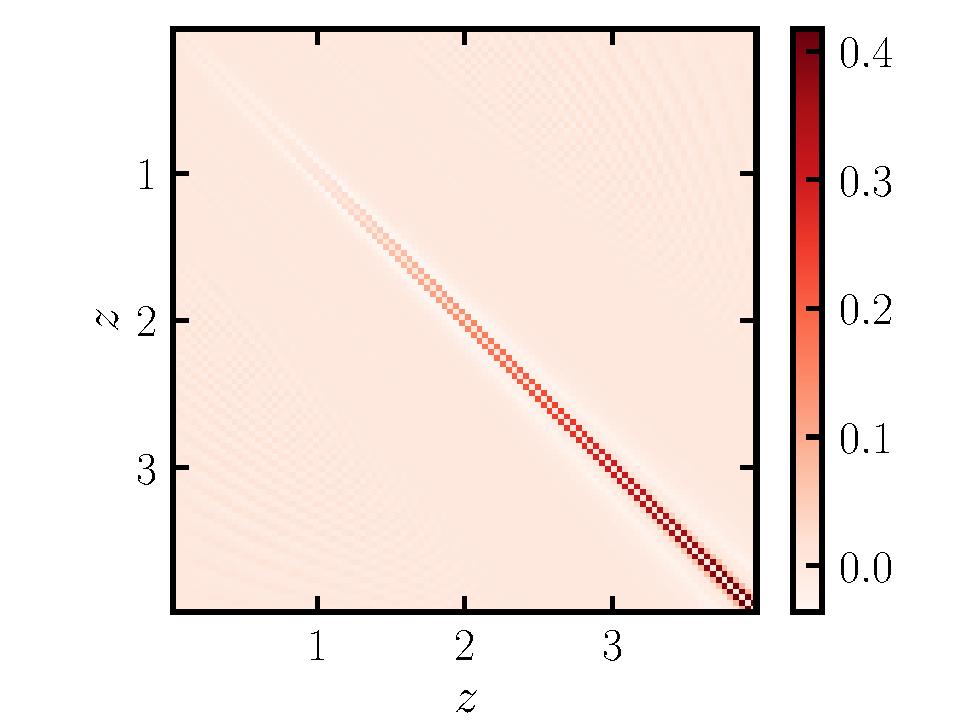
\includegraphics[width=1.\textwidth]{./corr_CV_0}
          \caption{Correlation matrix associated with the cosmic-variance contribution to the total $N(z)$ covariance for the first tomographic bin of the HSC data.}\label{fig:CV}
        \end{figure}
        The analysis presented in Section \todo{add ref} will make use of a measured redshift distribution estimated from the COSMOS 30-band catalog \todo{add ref}, as was done in \todo{add cite}. The main sources of uncertainty for this measurement are cosmic variance in the COSMOS field, shot noise and additional uncertainty in the photometric redshifts used to assign galaxies to different bins. Here we will associate each of this sources to a separate covariance that will be added in quadrature to form the final ${\sf C}_N$.
        
        The contribution from the photometric redshift systematic uncertainties is modelled as \ldots\todo{Not sure how you guys implemented this.}
        
        The cosmic variance uncertainties are caused by the fluctuations in the matter density traced by galaxies in the particular sky patch. The corresponding covariance would ideally be estimated from simulations including both non-linear gravitational clustering and a realistic model of the galaxy-halo connection for the specific galaxy sample under study. For simplicity in this proof-of-concept analysis we instead use an analytical model for the $N(z)$ covariance. Although less precise than a simulation-based calculation, this approach was shown by \todo{cite sanchez} to provide a reasonable prediction for the redsthift distribution uncertainties.

        The covariance matrix element between $N^\alpha_i$ and $N^\beta_j$ two tomographic bins is given by:
        \begin{equation}\label{eq:nz_cv}
          {\sf C}_{N,{\rm CV}}^{(i\,\alpha),(j\,\beta)}=\frac{N^\alpha_iN^\beta_j}{2\pi^2} \int_0^\infty dk_\parallel \cos(k_\parallel(\chi_\alpha-\chi_\beta))\int_0^\infty dk_\perp k_\perp W_\alpha(k_\parallel,k_\perp)W_\beta(k_\parallel,k_\perp)P_{gg}({\bf k}),
        \end{equation}
        where $\chi_\alpha$ is the radial comoving distance to redshift $z_\alpha$, and we model the galaxy power spectrum using the Kaiser formula \todo{cite} accounting for redshift-space distortions:
        \begin{equation}
          P_{gg}({\bf k},z)=\left(b_g(z)+f(z)\frac{k_\parallel^2}{k^2}\right)^2\,P_{mm}(k,z),
        \end{equation}
        where $f(z)$ is the logarithmic growth rate and $b_g(z)$ is the linear galaxy bias. Following the results of \todo{cite}, appropriate for the magnitude-limited sample studied here, we assume a redshift dependence for $b_g$ given by $b_g(z) = 0.95/D(z)$, with $D(z)$ the linear growth factor. $P_mm(k)$ is the non-linear matter power spectrum, which we model via the \todo{cite} HALOFIT parametrization.

        The overlapping deep HSC patch covering the COSMOS 30-band footprint used to measure the redshift distribution in this work covers a total area of $A_{\rm sky} = 1.7 \ {\rm deg}^2$. Modelling this patch as a disc of radius $\theta_{\rm sky}=0.73^\circ$, the corresponding window function in Eq. \ref{eq:nz_cv} is given by
        \begin{equation}
          W_\alpha(k_\parallel,k_\perp)=j_0(k_\parallel\Delta\chi_\alpha/2)\,\frac{2 J_1(k_\perp \chi_\alpha\theta_{\rm sky})}{k_\perp \chi_\alpha\theta_{\rm sky}},
        \end{equation}
        where $\Delta\chi_\alpha$ is the comoving width of the $\alpha$-th histogram bin, $j_0$ is the zero-th order spherical Bessel function and $J_1$ is the order-1 cylindrical Bessel function.

        We assume that the cosmic covariance between the tomographic bins is negligible, so we estimate the cosmic variance covariance matrix by treating each bin independently. We show the resulting correlation matrix of the COSMOS cosmic variance in Fig. \ref{fig:CV}.
        
        The final contribution, from shot noise, is caused by the discrete nature of galaxies as a tracer of the matter fluctuations, and is simply given by
        \begin{equation}
          {\sf C}^{(i\,\alpha),(j\,\beta)}_{N,{\rm SN}}=\delta_{\alpha\beta}\delta_{ij}N^\alpha_i.
        \end{equation}
        We find this contribution to be subdominant in all cases in comparison with cosmic variance.

    \subsubsection{External priors and smoothness}\label{sssec:theory.prior.smooth}
      In addition to information from direct measurement of the $N(z)$, it is reasonable to impose certain properties on the underlying true reshift distributions based on physical considerations. For instance, there is no reason to expect that the physics of galaxy formation should generate sharp features in the redshift evolution of the abundance of galaxies. The transition of features in the spectra of different galaxy types between photometric bands at different redshifts could induce smaller-scale fluctuations in the $N(z)$. However, for a sufficiently diverse galaxy sample, one would not expect such fluctuations on scales $\delta z\lesssim0.04$ (corresponding to $\sim100\,{\rm Mpc}$ or $\sim0.2\,{\rm Gyr}$ at $z\sim1$). It is therefore a reasonable proposition to impose a certain degree of smoothness on the redshift distributions, which can be achieved through a purposely defined Gaussian prior. Applying these types of priors is admittedly a subjective choice to some extent, and we will study its impact on our results in Section \todo{ref}.
      
      One common way to impose smoothness on a function $f(x)$ is to penalize large values of its firs derivative via $p(f)\propto\exp\left[-(f'(x))^2/(2\sigma_1^2)\right]$. In the discrete formalism used here, this is equivalent to imposing a Gaussian prior on $\vN$ with zero mean ($\vN_P=0$) and an inverse covariance given by:
      \begin{equation}\label{eq:prior_1st}
        {\sf C}^{-1}_P=\frac{1}{\sigma_1^2}\sum_\alpha {\bf v}^{1T}_\alpha{\bf v}^1_\alpha,
      \end{equation}
      where
      \begin{equation}
        ({\bf v}^1_\alpha)_\beta=\left\{
        \begin{array}{ll}
          1  & {\rm if}\,\,\, \alpha=\beta+1\\
          -1  &  {\rm if}\,\,\, \alpha=\beta\\
          0 & {\rm otherwise}
        \end{array}\right.
      \end{equation}
      To understand this, note that, using finite differences, the derivative of $\vN$ is approximately $\vN'\propto {\bf v}^{1T}\vN$.

      The prior in Eq. \ref{eq:prior_1st} effectively penalizes large deviations between adjacent elements of $\vN$. This can be generalized to include all element pairs as
      \begin{equation}\label{eq:smooth1}
        {\sf C}^{-1}_P=\sum_{n=1}\sum_{\alpha}p_n\,{\bf v}^{n\,T}_\alpha{\bf v}^n_\alpha,
      \end{equation}
      where
      \begin{equation}
        ({\bf v}^n_\alpha)_\beta=\left\{
        \begin{array}{ll}
          1  & {\rm if}\,\,\, \alpha=\beta+n\\
          -1  &  {\rm if}\,\,\, \alpha=\beta\\
          0 & {\rm otherwise}
        \end{array} \right..
      \end{equation}
      The prefactor $p_n$ penalizes differences between neighbors of order $n$, and should therefore be a monotonically decreasing function of $n$ (since there should be no correlation between widely separated histogram bins). We therefore choose a functional form
      \begin{equation}
        p_n=A\,{\rm exp}\left[-\frac{1}{2}\left(n\frac{\Delta z}{\Delta z_{\rm thr}}\right)^2\right],
      \end{equation}
      where $\Delta z$ is the redshift separation between neighbouring histogram bins, and $\Delta z_{\rm thr}$ marks the redshift separation beyond which the $N(z)$ is expected to be uncorrelated. In our analysis we choose $A$ and $\Delta z_{\rm thr}$ as \todo{describe and motivate this}.
      
      %Determination of the prior matrix $P$ is where the the actual and often partially subjective prior on our knowledge of $N(z)$ enters. Note that the standard parameterizations can always be recast in this language at least in the perturbative limits. For example, a vector of derivatives $\lambda_i = dN_i/dz$ when added to $\vN$ will produce a shift in the the shape of $N_i(z)$. Therefore, adding a contribution $\sigma_{zi}^2 \lambda_i \lambda_i^T$ will allow shifts with variance $\sigma_{zi}$. Of course, when shifts become so large that the perturbative expansion breaks, the approach will work only approximately. But in this paper we are not interesting in shifts; instead we will try to build $P$ is a more systematic manner.

  \section{Appplication to HSC clustering data}\label{sec:hsc}
    \an{Some citations are currently missing but I will put them in later.}
    We apply the method outlined above to the data obtained in Ref.~\cite{1912.08209}. This work measured the angular galaxy clustering power spectrum from HSC DR1 data. In the following, we give a very brief summary of the methodology employed in this work and refer the reader to Ref.~\cite{1912.08209} for more details.
    \subsection{Background theory}\label{ssec:hsc.theory}
      The angular clustering power spectrum for galaxies in redshift bins $i$, $j$ with can be modeled using the Limber approximation as \cite{1953ApJ...117..134L, 1992ApJ...388..272K, Kaiser:1998}
      \begin{equation}\label{eq:cell_gg_limber}
        C^{ij}_\ell = \int \mathrm{d}z\,\frac{H(z)}{\chi^2(z)} p^i(z)p^j(z)\,P_{gg}\left(z,k=\frac{\ell+1/2}{\chi(z)}\right),
    \end{equation}
    where $P_{gg}(z,k)$ denotes the underlying 3D galaxy power spectrum, $\chi(z)$ is the comoving distance and $H(z)$ denotes the Hubble parameter at redshift $z$. $p^i(z)$ is the redshift probability distribution of bin $i$ normalized to unit area, and is therefore related to the unnormalized distribution via
    \begin{equation}
      p^i(z)=\left[\int dz N_i(z)\right]^{-1}N(z)=\frac{\sum_\alpha N^\alpha_i\phi_\alpha(z)}{\sum_\alpha N^\alpha_i\int dz\phi_\alpha(z)}.
    \end{equation}
    The simplicity with which the redshift distribution enters the prediction for the angular power spectrum in Eq.~\ref{eq:cell_gg_limber}, facilitates the computation of the ${\sf T}$ matrix defined above. 

    Finally, following Ref.~\cite{1912.08209} we estimate the theoretical prediction for the galaxy power spectrum $P_{gg}(z,k)$ within the halo model combined with halo occupation distribution modeling \cite{2000MNRAS.318.1144P,2002PhR...372....1C,2002ApJ...575..587B,2005ApJ...633..791Z,2013MNRAS.430..725V}. Details about HOD parameterizations can be found in these references, and we only provide a succinct description relevant to the present analysis here
    
    The galaxy power spectrum receives contributions from the so-called 1-halo and 2-halo terms:
    \begin{equation}
      P_{gg}(z,k) = P_{gg,{\rm 1h}}(z,k) + P_{gg,{\rm 2h}}(z,k),
    \end{equation}
    where
    \begin{align}
      & P_{gg,{\rm 1h}}(k)=\frac{1}{\bar{n}_g^2} \int \mathrm{d}M\,\frac{\mathrm{d}n}{\mathrm{d}M} \bar{N}_c\,\left[\bar{N}_s^2u_s^2(k)+2\bar{N}_su_s(k)\right],\\
      & P_{gg,{\rm 2h}}(k)=\left(\frac{1}{\bar{n}_g} \int \mathrm{d}M\,\frac{\mathrm{d}n}{\mathrm{d}M}\,b_h(M)\,\bar{N}_c\,\left[1+\bar{N}_su_s(k)\right]\right)^2\,P_{\rm lin}(k).
    \end{align}
    
    Here, $\mathrm{d}n/\mathrm{d}M$ is the halo mass function for halo mass $M$, $b_h(M)$ is the linear halo bias, $N_c(M)$ and $N_s(M)$ are the mean number of central and satellite galaxies in halos of mass $M$, $u_s(k)$ is the Fourier transform of the satellite density profile, and $P_{\rm lin}(k)$ is the linear matter power spectrum. The number density of galaxies is calculated as 
    \begin{equation}
      \bar{n}_g=\int \mathrm{d}M\,\frac{\mathrm{d}n}{\mathrm{d}M}\bar{N}_c(M)\left[1+\bar{N}_s(M)\right].
      \label{eq:ng_hod}
    \end{equation}    
    
    As in \cite{1912.08209}, we parametrize the number of centrals and satellites as a function of mass as:
    \begin{align}
      &\bar{N}_c(M)=\frac{1}{2}\left[1+{\rm erf}\left(\frac{\log_{10}(M/M_{\rm min})}{\sigma_{\log M}}\right)\right],\\
      &\bar{N}_s(M)=\Theta(M-M_0)\left(\frac{M-M_0}{M_1'}\right)^\alpha,
    \end{align}
    where $\Theta(x)$ is the Heavyside step function, and we model the distribution of satellites to follow that of the dark matter, given by a truncated Navarro-Frenk-White profile \cite{Navarro:1996}. The choices of mass function parametrization, halo bias and concentration-mass relation used here follow the same models used in \cite{1912.08209}, namely the mass function and halo bias of \cite{Tinker:2010}, and the concentration-mass relation of \cite{Duffy:2008} for a spherical overdensity halo masses with an overdensity parameter $\Delta=200$ with respect to the matter density.
 
    The HOD model is defined by three characteristic masses, $M_{\rm min}$, $M_0$ and $M_1$. We model the redshift dependence of these masses as a linear Taylor expansion in the scale factor around the mean redshift of the sample $z_p=0.65$ as
    \begin{equation}
      \log_{10}{M_x(z)} = \mu_x + \mu_{x, p} \left(\frac{1}{1+z} - \frac{1}{1+z_{p}}\right).
    \end{equation}
    where $x$ is $\mathrm{min}$, 0 or 1.
    
    Besides these HOD parameters, the analysis of \cite{1912.08209} marginalized over uncertainties in the redshift distribution using the shift-width parametrization of Eq. \ref{eq:photo-z-model}, including two additional shift and width parameters per redshift bin. For the four redshift bins described in section \todo{ref}, the complete set of 14 free parameters is
    \begin{equation}
      \vec{\theta}=\{\mu_{\rm min},\,\mu_{{\rm min},p},\,\mu_0,\,\mu_{0,p},\,\mu_1,\,\mu_{1,p},\,\Delta z_{\{1,2,3,4\}},\,z_{w,\{1,2,3,4\}}\}.
    \end{equation}

\subsection{The HSC dataset}
The Hyper-Suprime Cam survey is an on-going photometric galaxy survey survey focused mainly on weak gravitational lensing. The analysis in Ref.~\cite{1912.08209} is based on the publicly-available HSC DR1 data, whose so-called wide fields cover approximately 108 square degrees on the sky, subdivided into seven distinct patches. Ref.~\cite{1912.08209} used these data to compute spherical harmonic galaxy clustering power spectra for four tomographic redshift bins between $z=0.15$ and $z=1.5$, taking both auto- and cross-correlations into account. These power spectra have been corrected for observational and extragalactic systematics by deprojection at the map-level \cite{2019MNRAS.484.4127A}. Finally, following Ref.~\cite{2019PASJ...71...43H}, photometric redshift distributions have been estimated by cross-matching HSC galaxies to galaxies in the COSMOS 30-band photometric catalog presented in Ref.~\cite{2016ApJS..224...24L}.
\subsection{Validating the linear expansion}


\begin{figure}[ht]
\centering  
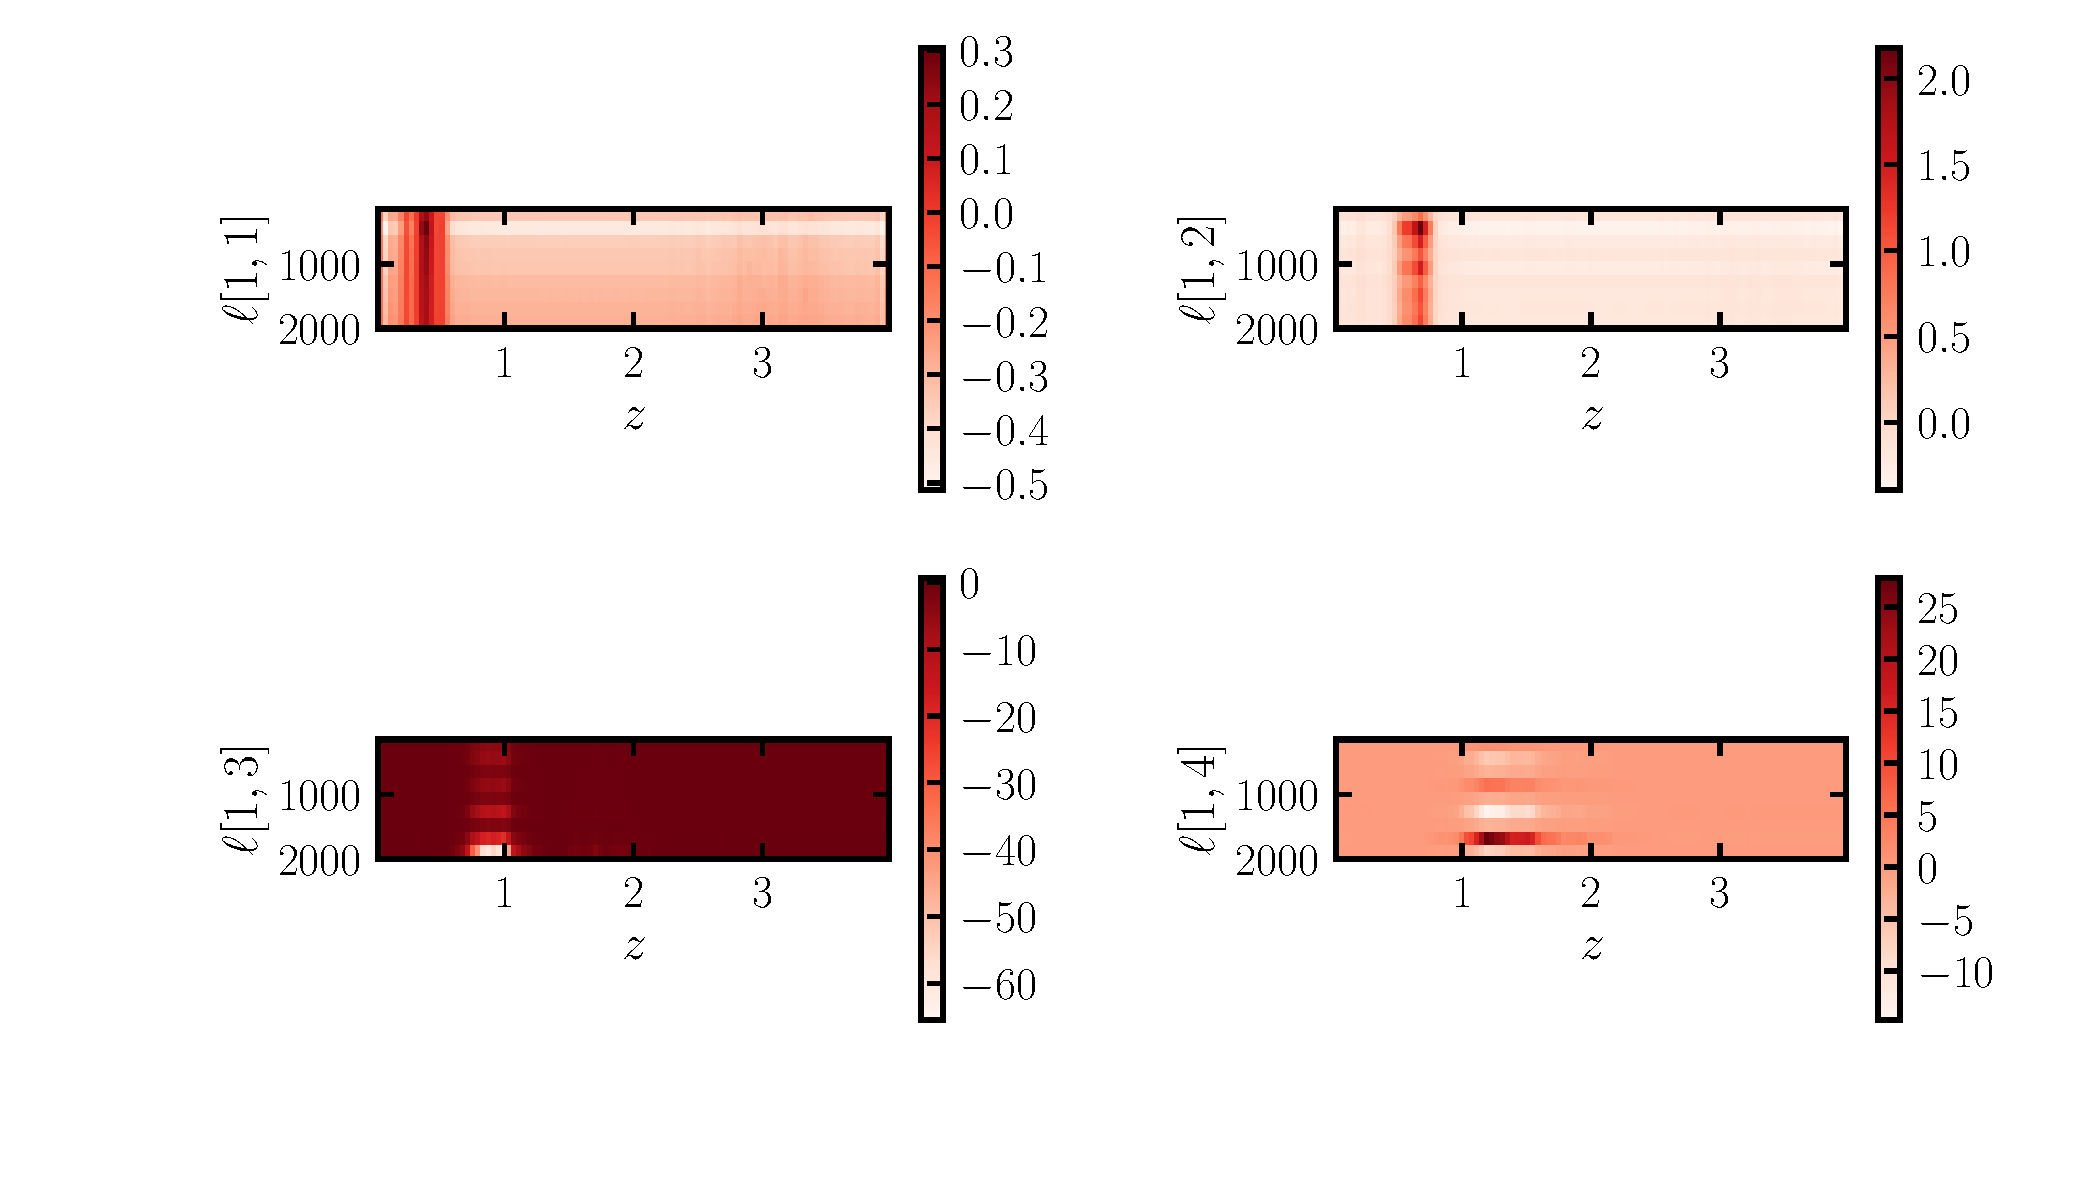
\includegraphics[width=1.\textwidth]{./Tmat}
\caption{Visualization of the derivative matrix $T_{mn} = {\partial t_m}/{\partial N_n}$. \todo{Make look nicer: split into tomo bins}} 
\label{fig:Tmat}
\end{figure}

\begin{figure}[ht]
\centering  
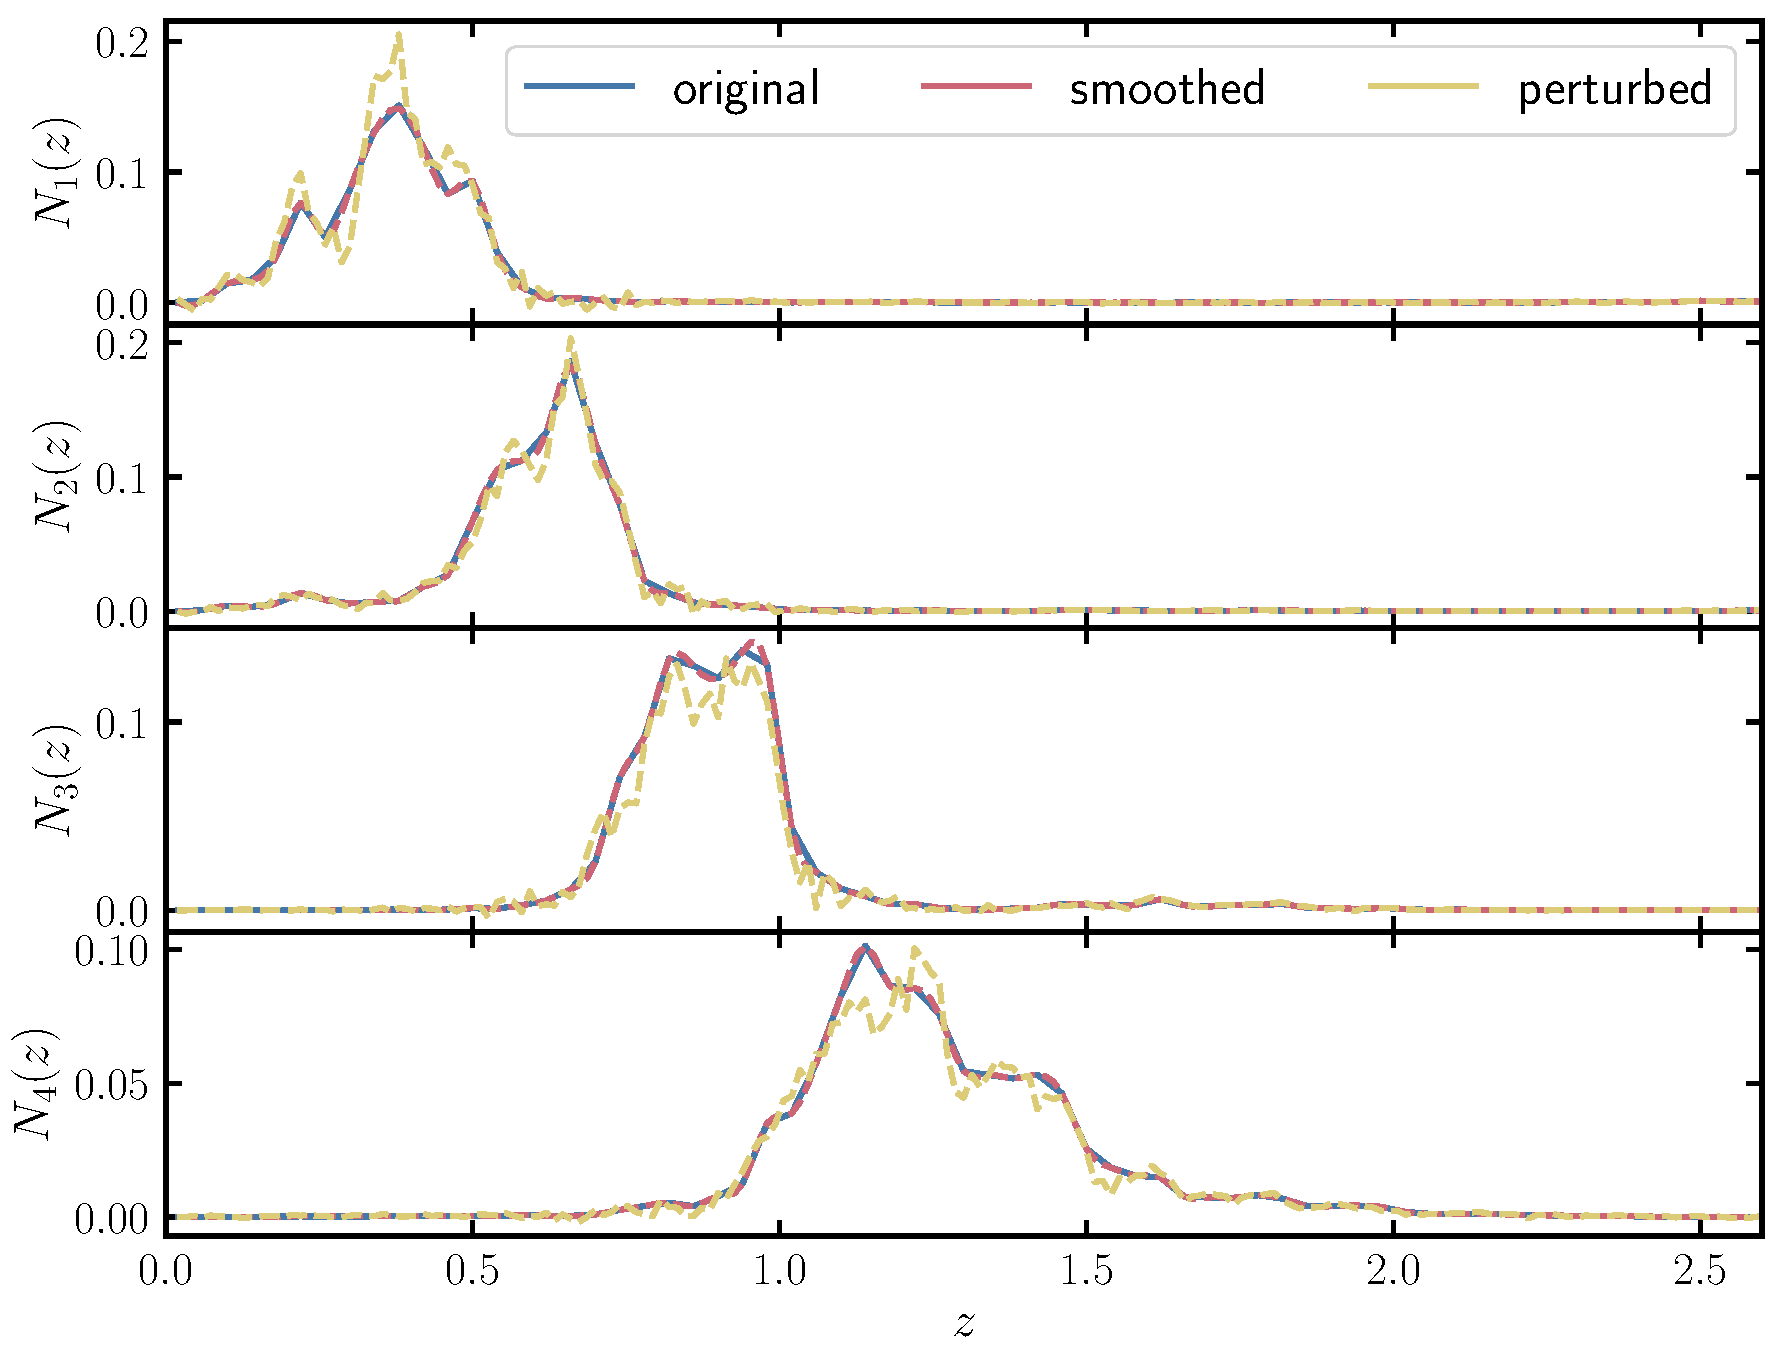
\includegraphics[width=1.\textwidth]{./Nzs}
\caption{Photometric redshift
distributions $N(z)$
of the four tomographic HSC bins.
The \textit{red} curves show the
default values used in the 
full HSC analysis (CITE Andrina),
while the \textit{blue} curves 
show their smoothed and upsampled 
version used in this work. The
\textit{green} show a random 
Gaussian draw from the smoothing 
prior described in Section TODO: Section}
\label{fig:Nzs}
\end{figure}

\begin{figure}[ht]
\centering  
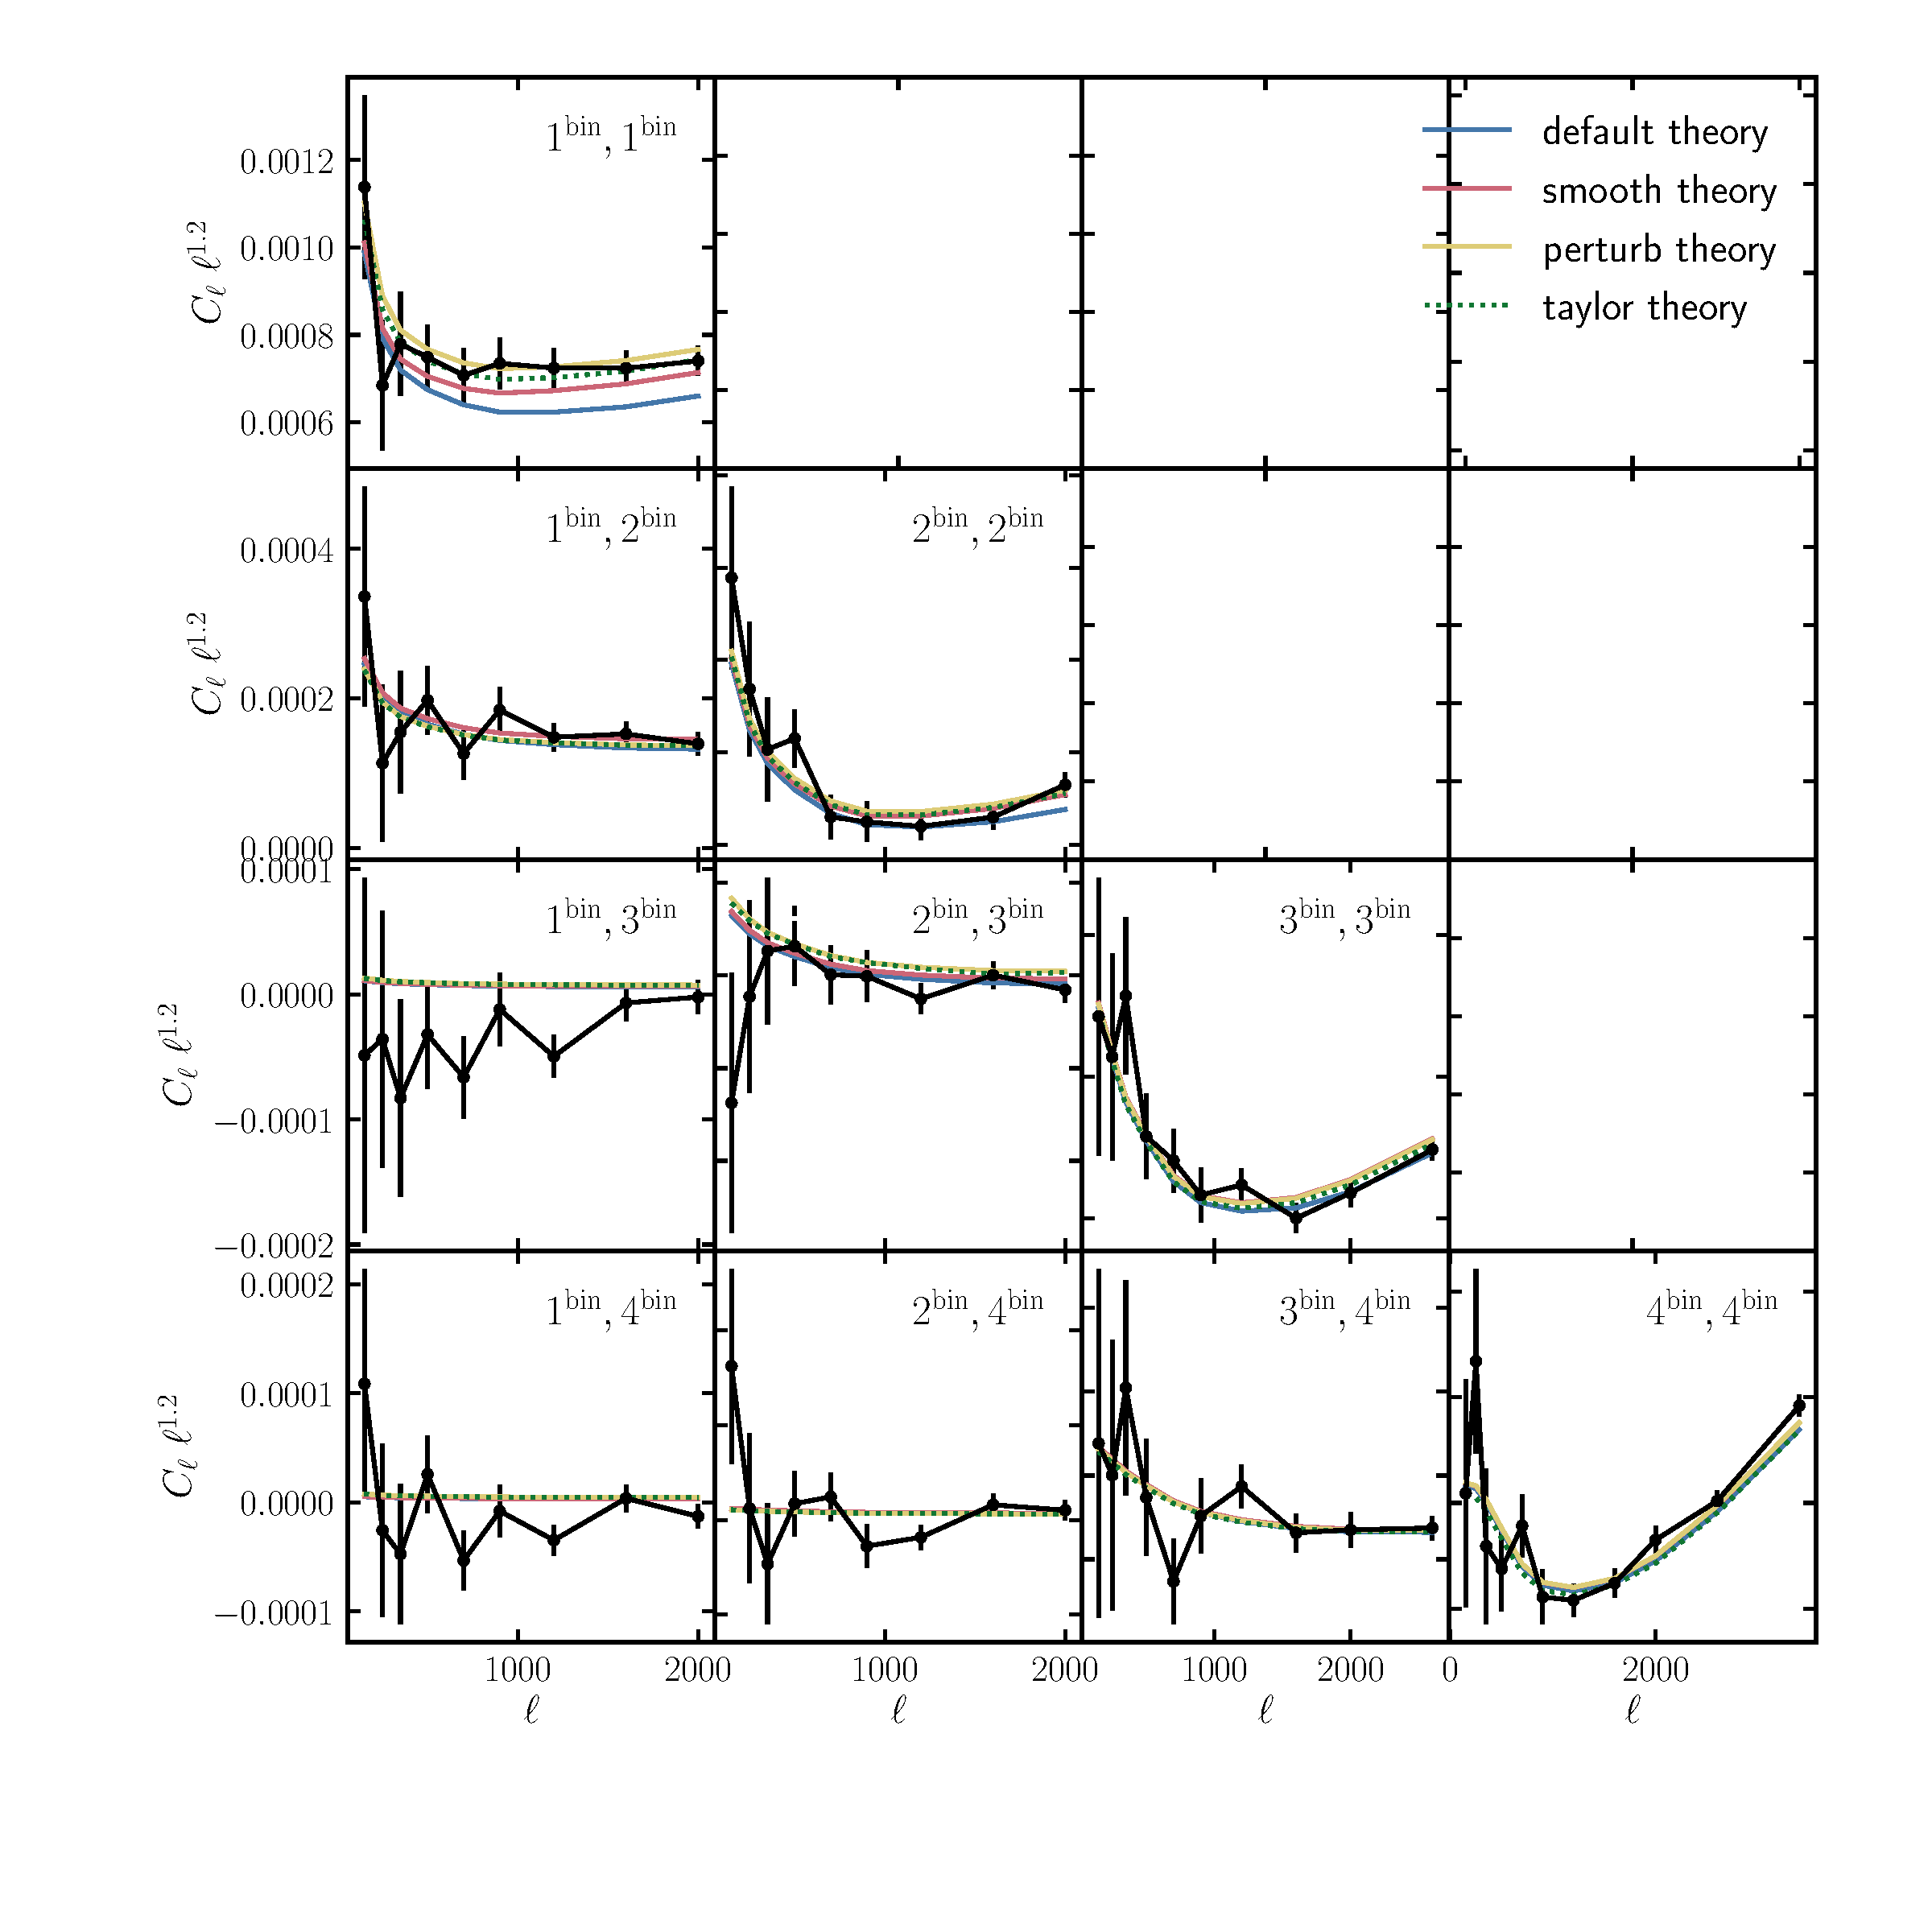
\includegraphics[width=1.\textwidth]{./Cls}
\caption{Galaxy power spectrum, $C_\ell^{gg}$, between the four
tomographic bins. The \textit{black} curves show the HSC-measured
power spectrum and error bars, while the
\textit{red} curves present the $C_\ell$s
computed using the posterior mean values of the 6 HOD parameters from the
full HSC analysis (CITE Andrina). In 
\textit{green} is shown the power
spectrum obtained by using the smoothed
$N(z)$ distributions (see Fig. \ref{fig:Nzs}). The \textit{blue}
curves correspond to the exact
calculation of the $C_\ell$s using the
perturbed $N(z)$ values in
Fig. \ref{fig:Nzs}, and the 
\textit{lightblue} dotted lines
show the power spectra derived via
Taylor expansion: $C_\ell' = C_\ell +
 {\sf T} \left(\vN' - {\vN} \right)$.}
\label{fig:Cls}
\end{figure}

\begin{table}
\begin{center}
 \begin{tabular}{c | c c } 
 \hline\hline
 Model & HSC cov. & Marginalized $N(z)$ cov. \\ [0.5ex] 
 \hline
  $\chi^2$, original $N(z)$, evaluated at $C_\ell$ & 98.97 & 88.97 \\ 

 $\chi^2$, smoothed $N(z)$, evaluated at $C_\ell$ & 91.33 & 86.44 \\

 $\chi^2$, perturbed $N(z)$, evaluated at $C_\ell'$ & 99.78 & 89.57 \\

 $\chi^2$, perturbed $N(z)$, taylor-expanded $C_\ell +
 {\sf T} \Delta \vN$ & 100.62 & 89.64 \\
 
 \hline
 \hline
\end{tabular}
\end{center}
\label{tab:lin}
\caption{$\chi^2$ values with respect to the HSC data of the four curves shown in Fig. \ref{fig:Cls}. $[\mu_1, \ \mu_{1,p}] =  [13.05, 0.79]$
Ratio of determinants of original precision to CV+noise+smooth precision per dof =  1.15
94}
\end{table}

Fig. \ref{fig:Nzs} shows the distribution of the
photometric redshifts of the HSC data

Fig. \ref{fig:Cls} displays the exact $C_\ell$ vs. 
linear prediction using the derivative matrix, ${\sf T}$.

In Fig. \ref{fig:Tmat}, we show the
derivative matrix, ${\sf T}$,
defined in Eq. \ref{eq:Tmat} for the first tomographic
bin in the HSC data and its cross-correlations with
all four bins, i.e. . The rows of the matrix correspond
to the $\ell$ multipoles, while the columns to the
redshift samples of $N(z)^1$.


\subsection{Impact of N(z) uncertainties on final parameters}
To study the effect on the covariance matrix
of the marginalization procedure described in detail
in sections TODO: CITE, we visualize the original
correlation matrix and its difference with the
marginalized matrix in Fig. \ref{fig:fid_marg_cov}. The
main effects on the original matrix is
a positive contribution to the off-diagonal entries
for redshift samples in close proximity. We set the free
parameters of our model to the following values: 
$A_{\rm smooth} = 1$, $A_{\rm noise} = 4.$,
$N_{\rm upsample} = 3$, and $\Delta z_{\rm thresh} = 
0.06$. These values were chosen so as to reduce the
$\chi^2$ of the perturbed model 
using the new covariance matrix when compared with the
original covariance matrix. The modest value of the
smoothing parameter, $A_{\rm smooth}$, ensure that we 
are not oversmoothing the $N(z)$ distribution, while
the choice of photometric noise as four times 
larger than the variance in the different photometric
measures provides a reasonable guess for the expected
variation in $N(z)$ given the uncertainty.

To assess whether the marginalization procedure 
proposed in this work provides better constraints
on the
6 HOD parameters than the original 14-parameter
model, we employ the ensemble sampler for Markov
chain Monte Carlo (MCMC) $\textsc{emcee}$ CITE Goodman 
\& Weare (2010) and other paper with 6 parameters and
a walkers' ratio of 6 for 12000 iterations. We assess
the convergence of the chains with a simple G-R test
having computed the auto-correlation and thinned the
chains beforehand. In all cases, we find that the
chains are reasonably well converged. 

In Fig. \ref{fig:fid_marg_cov}, we show the key 
comparison between

We can
see that the full analysis leads to 
worse constraints on the parameters
when compared with the marginalized
covariance. Furthermore, the proximity
of the \textit{blue} and \textit{red} 
contours serves both as a sanity check 
that our method yields physical constraints
of the 6 parameters (i.e. not exceeding
the cosmic variance limits) as well as 
nearly optimal such

We, furthermore, run the following several 
tests to check the robustness of our result:
\begin{itemize}
\item We study the effect of the smoothing
by turning it off, $A_{\rm smooth} = 0$. 
\item We vary the choice for the
diagonal photometric noise parameter
by increasing it to $A_{\rm noise} = 42$.
\item We compute the ${\sf T}$ matrix 
using a different set of 
HOD parameters perturbed by $1\sigma$
away from the fiducial ones.
\end{itemize}
We show these comparisons with the
fiducial marginalized $N(z)$ model in Fig.
\ref{fig:triangle_marg_tests}.
One can notice that the effect of the
smoothing on the constraints is minimal,
while increasing the diagonal noise
leads to weakening them. Neither of these
tests changes significantly the
mean of the posterior distribution.
On the other hand, offsetting the 
HOD parameters used in the ${\sf T}$
matrix computation leads to a shift to
the mean and a slight widening of the
contours. That is because the covariance
matrix used in the analysis no longer
favors the HOD values preferred by the
data. This slight tension
results in sub-par convergence
of the chains and shifted mean posteriors.

\ref{fig:triangle_fid_marg}
\begin{figure}[ht]
\centering
\begin{subfigure}{.5\textwidth}
  \centering
  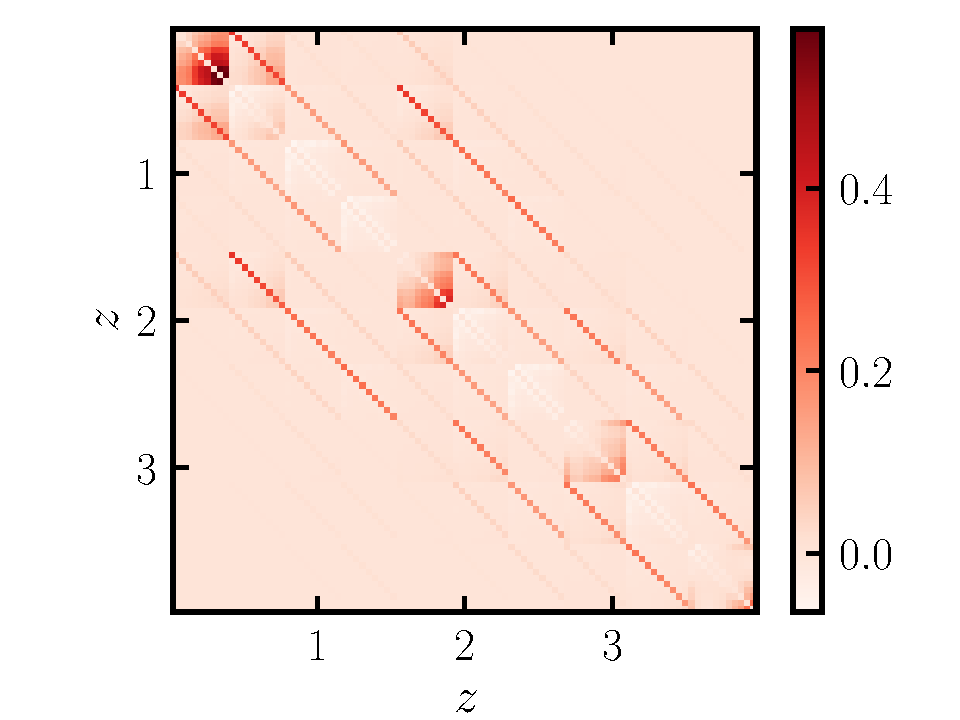
\includegraphics[width=1.\linewidth]{./corr_data}
\end{subfigure}%
\begin{subfigure}{.5\textwidth}
  \centering
  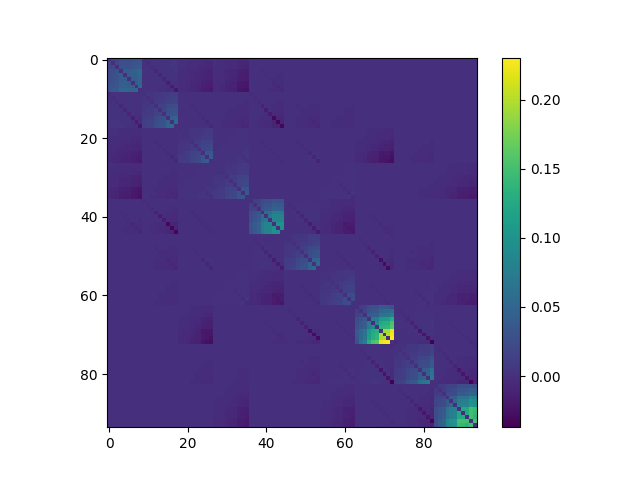
\includegraphics[width=1.\linewidth]{./corr_diff}
\end{subfigure}
\caption{Correlation matrix of the original HSC dataset (\textit{left} panel) and difference between the
original and the marginalized (this work)
correlation matrices (\textit{right} panel). Most of the
effect of marginalizing for the shift and width
parameters is manifested as a positive contribution
to the original matrix near the diagonal (i.e. there
is an increase in correlation for close redshift
values). Note that we have subtracted the diagonal
off the two matrices.}
\label{fig:fid_marg_cov}
\end{figure}

\begin{figure}[ht]
\centering  
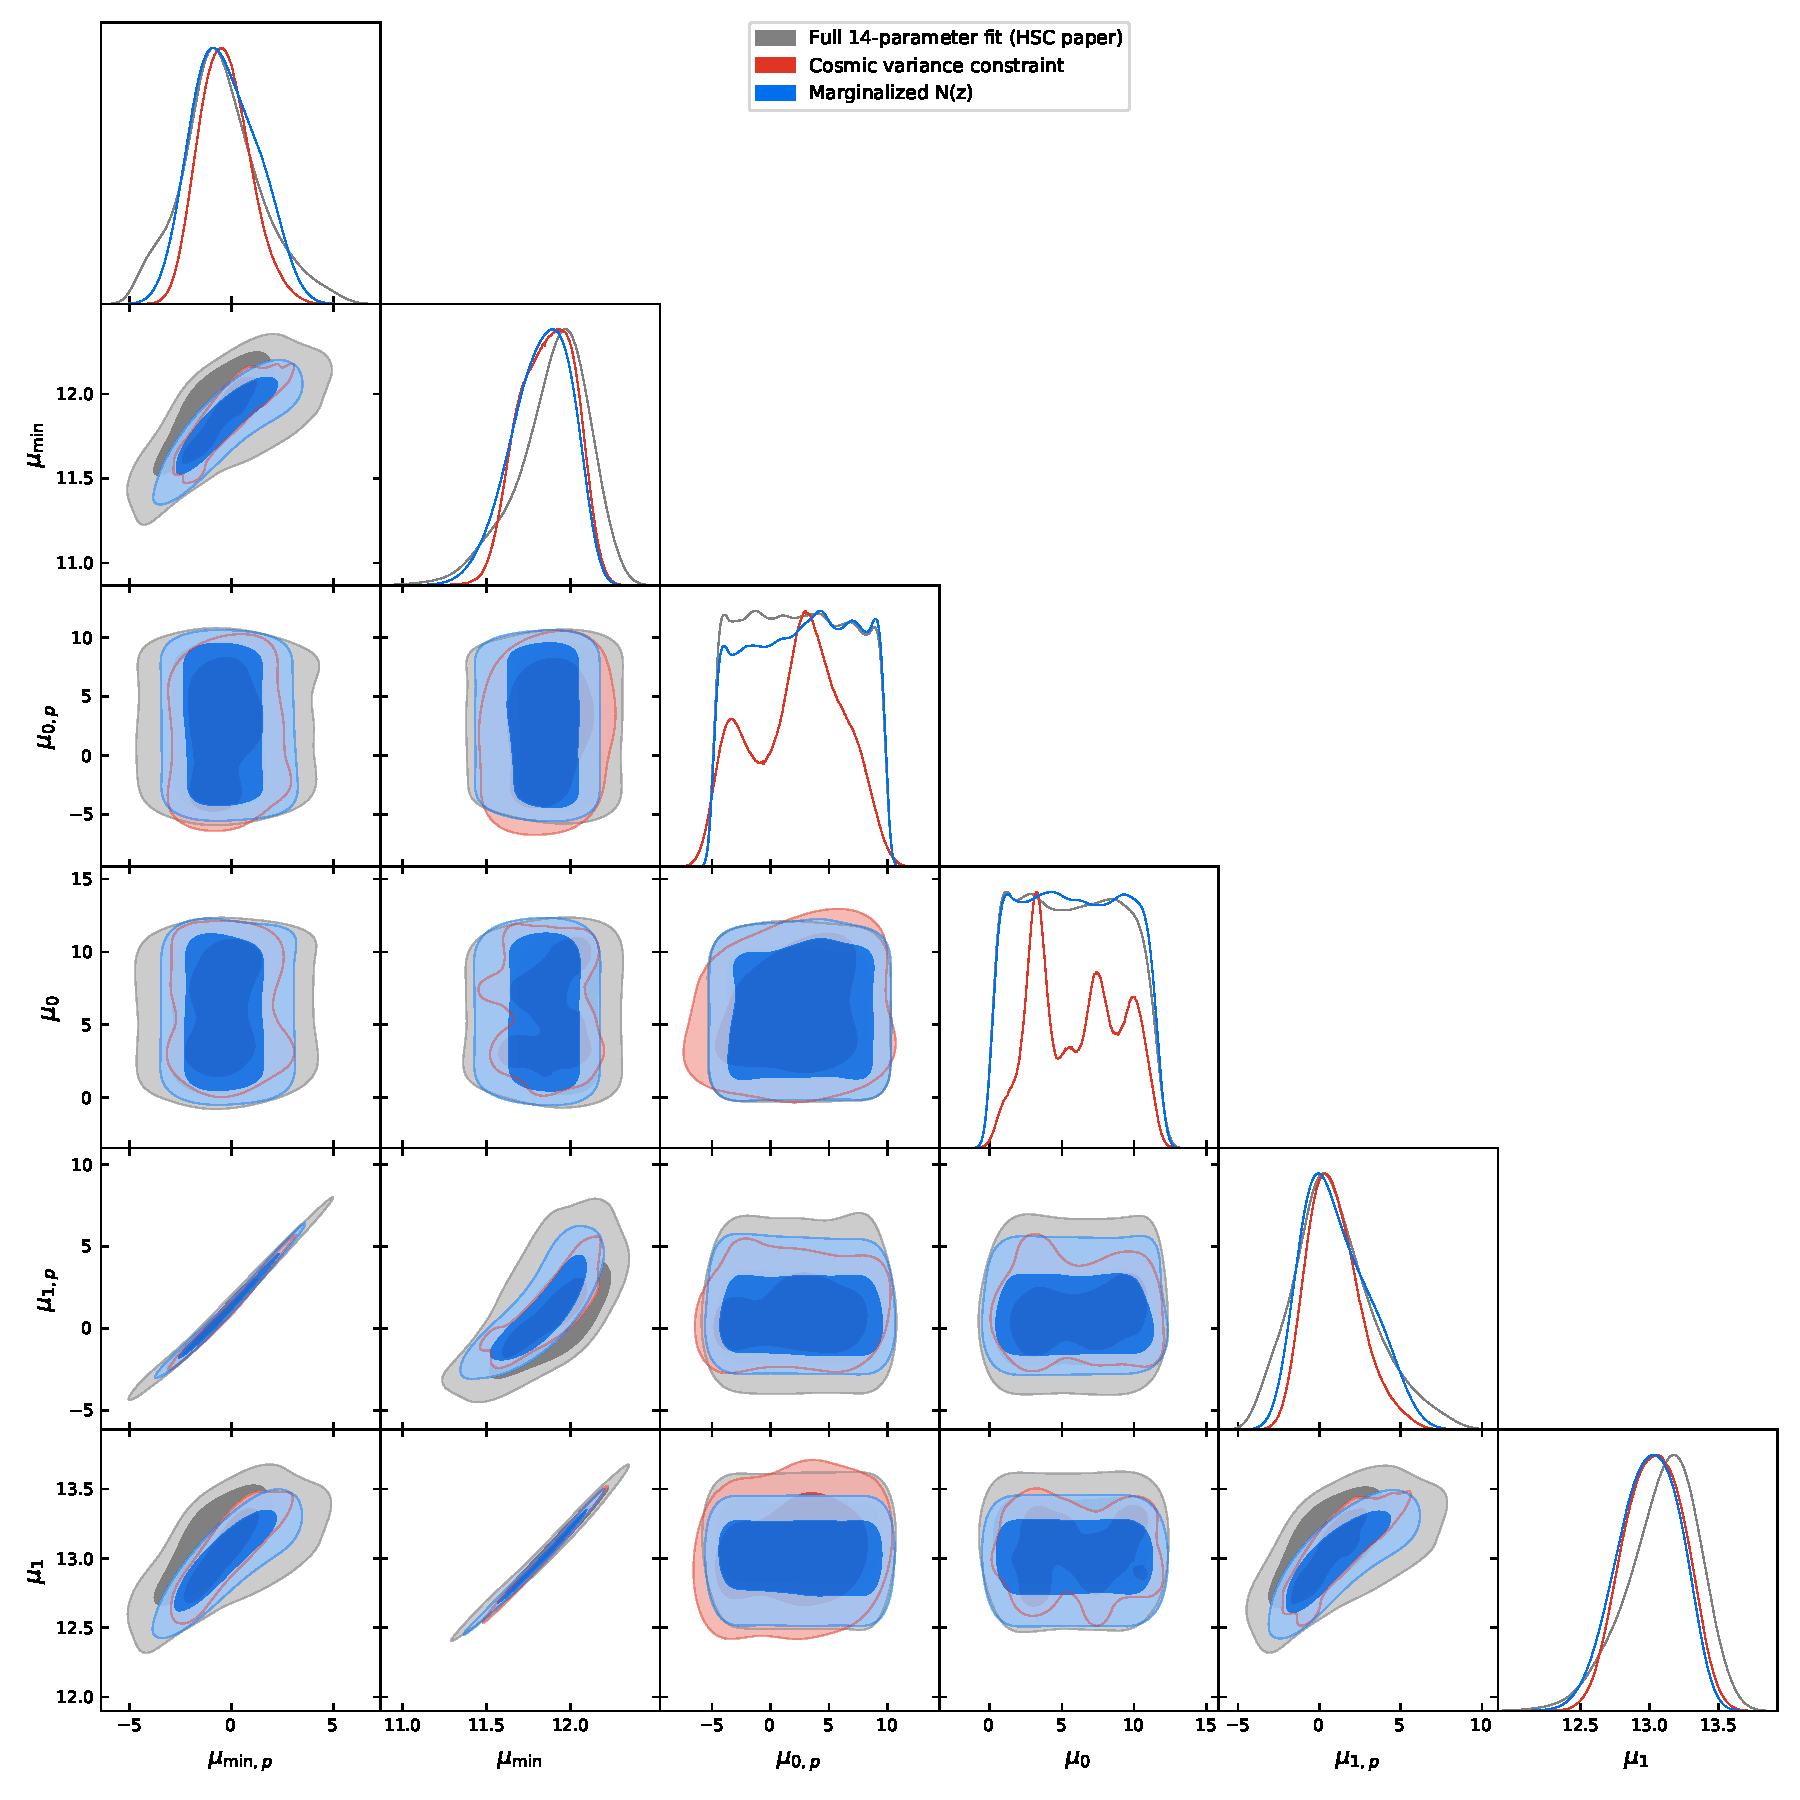
\includegraphics[width=1.\textwidth]{./triangle_fid_marg}
\caption{Triangle plot with constraints of 
the 6 HOD parameters obtained using the 
covariance matrix from the full
14-parameter original HSC analysis 
(\textit{gray contours}). The \textit{red
contours} are obtained by applying
importance sampling to the full original 
chain with weights determined by the
cosmic variance constraints of the
shift and width parameters. In \textit{blue},
we show the constraints on the 6 HOD parameters
obtained using the covariance
matrix marginalized to account for the
$N(z)$ uncertainty (i.e. without the
8 shift and width parameters). We can
see that the full analysis leads to 
worse constraints on the parameters
when compared with the marginalized
covariance.}
\label{fig:triangle_fid_marg}
\end{figure}

\begin{figure}[ht]
\centering  
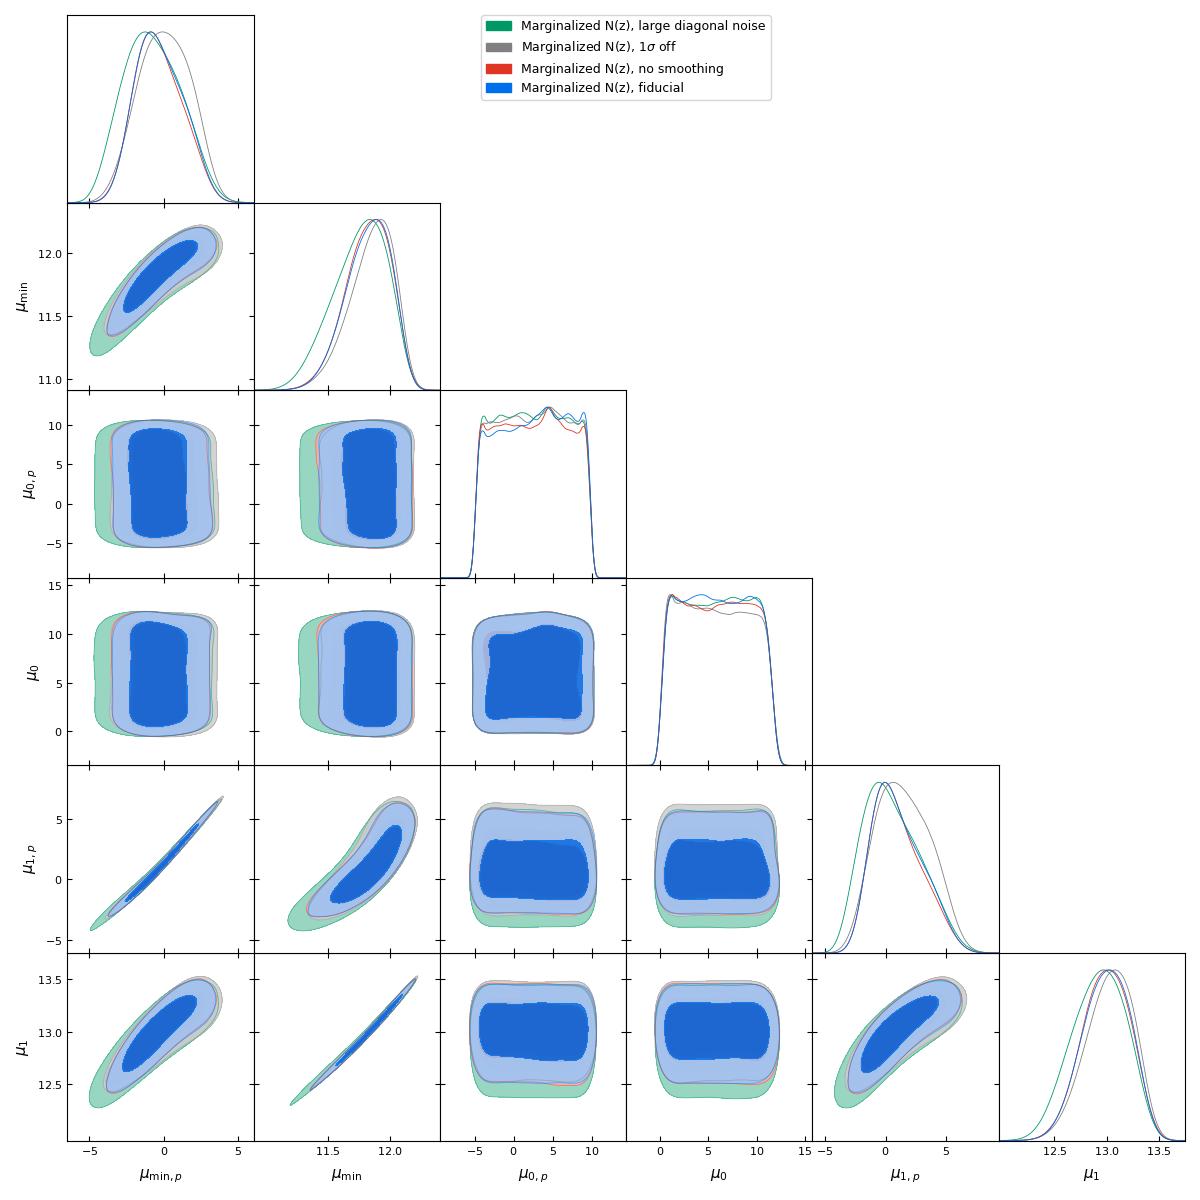
\includegraphics[width=1.\textwidth]{./triangle_marg_tests}
\caption{Triangle plot with constraints of the 6 HOD parameters obtained using different choices for the marginalized covariance matrix: in \textit{green}, we show the result where the diagonal noise is set to a very large value ($A_{\rm noise} = 42$); in \textit{gray} is shown the case where the marginalization is performed assuming fiducial HOD-model values which are $1\sigma$ away from their posterior mean values taken from \todo{CITE Andrina's paper}; in \textit{red}, we display the case where the smoothing has been removed ($A_{\rm smooth} = 0$); and finally the \textit{blue} contours show the fiducial case with $A_{\rm noise} = 4$ and $A_{\rm smooth} = 1$.}
\label{fig:triangle_marg_tests}
\end{figure}




\begin{table}
\begin{center}
\begin{tabular}{c | c c c c} 
 \hline\hline
 Parameter & HSC cov. [68\%, 95\%] & CV constraints [68\%, 95\%] & Marg. $N(z)$ [68\%, 95\%] \\ [0.5ex] 
 \hline
 $\chi^2/\nu$ & 87.49/80 & --- & 88.54/88 \\ 
$\mu_{{\rm min},p}$ & $-0.5^{+1.7}_{-2.0}$, $^{+4.0}_{-4.0}$ & $-0.4^{+1.1}_{-1.4}$, $^{+2.5}_{-2.3}$ & $-0.3^{+1.5}_{-1.8}$, $^{+3.2}_{-2.8}$ \\ [1ex]
$\mu_{\rm min}$ & $11.90^{+0.26}_{-0.15}$, $^{+0.39}_{-0.46}$ & $11.86^{+0.19}_{-0.16}$, $^{+0.28}_{-0.30}$ & $11.83^{+0.21}_{-0.15}$, $^{+0.32}_{-0.36}$ \\ [1ex]
$\mu_{0,p}$ & $2.4\pm 4.3$, $^{+7.2}_{-7.0}$ & $2.1^{+4.2}_{-5.1}$, $^{+6.6}_{-7.2}$ & $2.7^{+6.7}_{-4.4}$, $^{+6.9}_{-7.1}$ \\ [1ex]
$\mu_{0}$ & $5.7\pm 3.3$, $^{+5.5}_{-5.5}$ & $6.1^{+4.6}_{-3.8}$, $^{+5.2}_{-4.8}$ & $5.8\pm 3.4$, $^{+5.5}_{-5.5}$ \\ [1ex]
$\mu_{1,p}$ & $0.9^{+2.0}_{-2.8}$, $^{+5.1}_{-4.7}$ & $0.9^{+1.3}_{-1.8}$, $^{+3.4}_{-2.9}$ & $1.0^{+1.6}_{-2.6}$, $^{+4.1}_{-3.5}$ \\ [1ex]
$\mu_{1}$ & $13.10^{+0.30}_{-0.21}$, $^{+0.48}_{-0.54}$ & $13.04\pm 0.21$, $^{+0.38}_{-0.40}$ & $13.00^{+0.25}_{-0.21}$, $^{+0.42}_{-0.44}$ \\ [1ex]
 \hline
 \hline
\end{tabular}
\end{center}
\label{tab:chi2_tests}
\caption{Table showing the minimum
$\chi^2$ value as well as the 68\% and 95\% constraints on the 6 HOD parameters
in three regimes: using the original
HSC covariance matrix with 14 parameters (6 HOD + 8 $N(z)$ ones),
importance-sampling the original
chain to get cosmic variance constraints on the parameters, and finally using the
marginalized $N(z)$ covariance matrix with the 6 HOD parameters developed in this work.}
\end{table}

\begin{table}
\begin{center}
\begin{tabular}{c | c c c c} 
 \hline\hline
 Parameter & Fiducial [68\%, 95\%] & Test 1 [68\%, 95\%] & Test 2 [68\%, 95\%] & Test 3 [68\%, 95\%] \\ [0.5ex] 
 \hline
 $\chi^2/\nu$ & 88.54/88 & 87.67/88 & 88.56/88 & 78.61/88 \\ 
$\mu_{{\rm min},p}$ & $-0.3^{+1.5}_{-1.8}$, $^{+3.2}_{-2.8}$ & $0.0\pm 1.7$, $^{+3.2}_{-3.3}$ & $-0.3^{+1.4}_{-1.8}$, $^{+3.2}_{-2.8}$ & $-0.8^{+1.8}_{-2.1}$, $^{+3.7}_{-3.5}$ \\ [1ex]
$\mu_{\rm min}$ & $11.83^{+0.21}_{-0.15}$, $^{+0.32}_{-0.36}$ & $11.85^{+0.22}_{-0.13}$, $^{+0.31}_{-0.37}$ & $11.83^{+0.21}_{-0.15}$, $^{+0.33}_{-0.36}$ & $11.76^{+0.26}_{-0.17}$, $^{+0.38}_{-0.43}$ \\ [1ex]
$\mu_{0,p}$ & $2.7^{+6.7}_{-4.4}$, $^{+6.9}_{-7.1}$ & $2.5\pm 4.3$, $^{+7.1}_{-7.1}$ & $2.5\pm 4.3$, $^{+7.1}_{-7.1}$ & $2.5\pm 4.3$, $^{+7.1}_{-7.1}$ \\ [1ex]
$\mu_{0}$ & $5.8\pm 3.4$, $^{+5.5}_{-5.5}$ & $5.8^{+3.6}_{-5.2}$, $^{+5.6}_{-5.5}$ & $5.8\pm 3.4$, $^{+5.5}_{-5.5}$ & $5.9\pm 3.4$, $^{+5.5}_{-5.6}$ \\ [1ex]
$\mu_{1,p}$ & $1.0^{+1.6}_{-2.6}$, $^{+4.1}_{-3.5}$ & $1.5^{+2.1}_{-2.6}$, $^{+4.3}_{-3.9}$ & $0.98^{+1.5}_{-2.5}$, $^{+4.2}_{-3.5}$ & $0.6^{+1.9}_{-2.9}$, $^{+4.6}_{-4.0}$ \\ [1ex]
$\mu_{1}$ & $13.00^{+0.25}_{-0.21}$, $^{+0.42}_{-0.44}$ & $13.03^{+0.26}_{-0.20}$, $^{+0.41}_{-0.45}$ & $13.00^{+0.25}_{-0.22}$, $^{+0.42}_{-0.44}$ & $12.93^{+0.29}_{-0.24}$, $^{+0.47}_{-0.50}$ \\ [1ex]
 \hline
 \hline
\end{tabular}
\end{center}
\label{tab:chi2_tests}
\caption{Table}
\end{table}



\section{Conclusions}

\appendix
\section{Oversampling}
We may want to sub-sample the originally measured $N_{\alpha}$ ($\alpha\in[0,N_z^{\rm coarse})$) into a finer grid $n_{\mu}$ ($\mu\in[0,N_z^{\rm fine})$). This is essentially interpolation, which we can write as a linear operator $n_\mu = O_{\mu\alpha}N_{\alpha}$. The CV covariance of the $n_\mu$ is then given by ${\rm Cov}^{\rm fine}_{\mu\nu}=O_{\mu\alpha}O_{\nu\beta}{\rm Cov}^{\rm coarse}_{\alpha\beta}$.

For nearest-neighbor interpolation, the kernel $O_{\mu\alpha}$ is simply $O_{\mu\alpha}=\delta_{\alpha\alpha_\mu}$, where $\alpha_\mu$ is the index of the $N_\alpha$ that lies closest to $n_\mu$. In practice, the easiest thing to do will be to just use the same linear interpolation function (e.g. scipy's {\tt interp1d}) on all the rows of ${\rm Cov}^{\rm coarse}$ and then all the columns of the resulting matrix.


\bibliography{bibliography}

\end{document}
